\documentclass[a4paper]{article}

\usepackage[dutch]{babel}
% \usepackage{fullpage}
\usepackage{graphicx}
\usepackage{url}

\newcommand{\casam}{C.A.S.A.M. }
\newcommand{\casamproject}{C.A.S.A.M.-pro\-ject }


\title{\casamproject Ori\"{e}ntatieverslag}
\author{S.E.F. van Berkel \and B. Bijl \and J.Y.T. den Hollander \and S. Rabbelier \and B.M.W. Sedee \and N.N. Smit}

\begin{document}

\begin{titlepage}

\maketitle

\thispagestyle{empty}

\end{titlepage}

\setcounter{page}{2}
\setcounter{tocdepth}{2}

\tableofcontents

\newpage

\section{Inleiding}
\label{inleiding}


\section{Projectbeschrijving}
\label{Projectbeschrijving}


\section{Software}
\label{Software}
In dit hoofdstuk bespreken we de softwaretechnologi/"{e}n die we gaan gebruiken om de applicatie te maken. 
We beginnen met de basis van de applicatie door eerst de IDE, Python en Django te bespreken. 
Hierna bespreken we de 2 gebruikte bibliotheken, VTK en PIL. 
Tot slot bespreken we kort JavaScript en Flash.

\subsection{Integrated Development Environment (IDE): Eclipse}
%TODO: Write something nice about Eclipse and PyDev? Any volunteers?

\subsection{Python}
%TODO: Sverre, go wild!

\subsection{Django}
%TODO: Sverre, go wild! Once again!

\subsection{Visualisation Toolkit (VTK)}
Voor het implementeren van de benodigde Image Processing Technieken maken we gebruik van de Visualisation Toolkit (VTK)\cite{vtk}. 
VTK is een open source toolkit voor 3D graphics. 
In ons geval zetten we de toolkit in voor 2D graphics. 
VTK bestaat uit een C++ class bibliotheek en onder andere een Python interface laag.\cite{vtk2} 
Er zitten uitgebreide mogelijkheden in op het gebied van Image Processing en visualisatie.
In de VTK zitten de benodigde filters om Generalized Procrustes Analysis en Principal Component Analysis uit te voeren. 
Verder bevat de toolkit een implementatie van de Thin Plate Spline transformatie. 
Door de z-co\"{o}rdinaten op 0 te zetten kan VTK in de 2D ruimte worden gebruikt. 

\subsection{Python Imaging Library (PIL)}
Om de wat simpelere Image Processing technieken te implementeren maken we gebruik van de Python Imaging Library (PIL)\cite{pil}. 
Er is een handbook beschikbaar waarin de functionaliteiten besproken worden.\cite{pilhandbook} 
Dit kan onder andere ingezet worden voor het resizen van images, puntoperaties, filtering, colour space conversies, rotatie en transformaties. 

\subsection{JavaScript}
Om een mooie en gebruiksvriendelijke user-interface te krijgen, gaan wij gebruik maken van JavaScript.
Hiervoor zijn er een aantal bibliotheken beschikbaar die ons gaan helpen (Scriptaculous\cite{scriptaculous} en Prototype\cite{prototype}).
Prototype gaan we onder andere gebruiken vanwege de mooie mogelijkheden om met AJaX om te gaan, en de handige manieren om objecten aan te maken.
De Scriptaculous bibliotheek biedt ons verschillende mogelijkheden voor visuele toepassingen binnen een website, zoals sliders en draggables

\subsection{Flash}
%TODO: Bastiaan, your expertise, show us it.


\section{Medische aspecten}
\label{Medische aspecten}


Om een brug te slaan tussen de kennis van de medici en de technici is het voor de technici van belang om te beschikken over een basale kennis van de relevante anatomie van het menselijk lichaam en de begrippen die gebruikt worden. We hebben ons verdiept in de veelgebruikte basistermen en de relevante anatomie van het been. In de opdracht werd een onderzoek als voorbeeld gebruikt betreffende de venen en zenuwen van het onderbeen. Het ging hierbij om lasertherapie behandeling van spataderen (varices). Varices ontstaan als de venenkleppen niet meer naar behoren functioneren en het bloed niet meer goed terug naar het hart wordt geleid. De vraagstelling van het onderzoek is hierbij, wat zijn de veilige gebieden om de laserbehandeling uit te voeren, oftewel waar ligt de nabijgegelegen zenuw ver genoeg van de vene af? Met dit onderzoek in het achterhoofd hebben we de relevante anatomische kennis erbij gezocht.
De onderstaande kennis komt uit de Atlas an de Anatomie van Sesam.\cite{sesam}

\subsection{Anatomie basisterminologie}

Voor het aangeven van gebieden in het lichaam worden in de medische wetenschap bepaalde basisbegrippen gebruikt. Allereerst kan het menselijk lichaam opgedeeld worden in de hoofdgebieden. 
Zo is er de stam (truncus) en de bovenste en onderste ledematen (extremiteiten). 
De stam bestaat uit het hoofd (caput), de hals (collum) en de romp. 
De romp zelf bestaat uit de borst (thorax), buik (abdomen) en bekken (pelvis). 
De grens tussen truncus en de extremiteiten bevinden zich aan de bovenzijde bij de schoudergordel en aan de onderzijde bij de bekkengordel. 
Vervolgens zijn er vlakken beschreven die een doorsnede van het menselijk lichaam beschrijven. Deze lopen door de drie hoofdassen van het lichaam. Allereerst is er de verticale of longitudinale as. Dit is de lengte-as van het lichaam. Ten tweede is er de transversale of horizontale as. Deze as staat loodrecht op de verticale as en loopt van links naar rechts door het lichaam. De derde as is de saggitale as. Deze as staat loodrecht op de eerste twee assen en loopt van achteren naar voren door het lichaam. 

Op basis van de eerdergenoemde assen zijn vlakken door het lichaam te defini\"{e}ren:
\begin{itemize}
	\item Mediaan of mediaan-saggitaal vlak: door lengte- en saggitale as
	\item Saggitaal of paramediaan vlak: evenwijdig aan mediaan vlak
	\item Frontaal of coronaal vlak: door transversale assen, loodrecht op mediaan-saggitaal vlak
	\item Transversale vlakken: loodrecht op mediaan vlak en een frontaal vlak
\end{itemize}

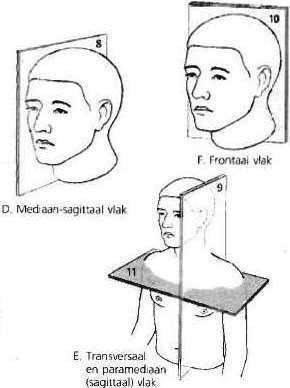
\includegraphics[width=0.9\textwidth]{sesam}

Om specifiekere gebieden aan te geven worden er een aantal termen gebruikt om een richting te omschrijven, hieronder een kort overzicht:
\begin{itemize}
	\item Craniaal: richting de schedel
	\item Superior/inferior: naar boven/naar beneden
	\item Mediaal/lateraal: naar het midden/van het midden af
	\item Centraal (profundus)/perifeer (superficialis): naar het inwendige/naar het oppervlakte
	\item Anterior/posterior: naar voren/naar achteren
	\item Proximaal/distaal: naar de bevestiging van de ledematen/ervan af
	\item Tibiaal/fibulair: naar het scheenbeen/naar het kuitbeen
	\item plantair : naar de voetzool toe
\end{itemize}

\subsection{Anatomie van het been}

Voor het begrip van de anatomie van het been bekijken we vervolgens de belangrijkste bot- vaat- en zenuwstructuren. 
Het gaat te ver om hier een uitgebreide beschrijving van te geven, wederom is slechts basiskennis benodigd. Wat betreft de botstructuren is er allereerst het bovenbeen (femur). De femur vormt de verbinding tussen de bekkengordel en de knie. Vervolgens is er de knieschijf (pattella) die het kniegewricht beschermd. In het onderbeen zijn het scheenbeen (tibia) en het kuitbeen (fibula) te vinden, deze vormen de verbinding tussen de knie en de enkel. In de voet bevinden zich vele botten, waarvan voor een ander onderzoek dat we gezien hebben het hielbeen (calcaneus) het meest relevant is. Belangrijke bony landmarks\footnote{landmarks die voortkomen uit de anatomie van het menselijk lichaam en voelbaar zijn vanaf de buitenkant} voor het onderbeen zijn onder andere de mediale en laterale malleolus. De mediale malleolus bevind zich aan de binnenzijde van de enkel en is een onderdeel van de tibia. De laterale malleolus bevindt zich aan de buitenzijde van de enkel en is een onderdeel van de fibula.

Wat betreft de vaatstructuren zijn er arteri\"{e}n en venen te onderscheiden. De vaatstructuren relevant voor het voorbeeldonderzoek bevinden zich in het onderbeen, het is met name de Vena Saphena Parva (VSP). Deze ontstaat aan de laterale voetrand en trekt door naar de Vena Poplitea, die zich bij de knie bevindt. De nabijgelegen zenuw die relevant is is de surale zenuw (Nervus Suralis) welke een vertakking is van de Nervus Tibialis.




\newpage
\bibliographystyle{plain}
\bibliography{Orientatie}

\end{document}

